%% file: template.tex = LaTeX template for article-like report 
%% init: sometime 1993
%% last: Feb  8 2015  Rob Rutten  Deil
%% site: http://www.staff.science.uu.nl/~rutte101/rrweb/rjr-edu/manuals/student-report/

%% First read ``latex-bibtex-simple-manual.txt'' at
%% http://www.staff.science.uu.nl/~rutte101/Report_recipe.html

%% Start your report production by copying this file into your XXXX.tex.
%% Small changes to the header part will make it an A&A or ApJ manuscript.

%%%%%%%%%%%%%%%%%%%%%%%%%%%%%%%%%%%%%%%%%%%%%%%%%%%%%%%%%%%%%%%%%%%%%%%%%%%%
\documentclass{aa}   %% Astronomy & Astrophysics style class

\usepackage{graphicx,natbib,url,twoopt}
\usepackage[varg]{txfonts}           %% A&A font choice
\usepackage{hyperref}                %% for pdflatex
%%\usepackage[breaklinks]{hyperref}  %% for latex+dvips
%%\usepackage{breakurl}              %% for latex+dvips
\usepackage{pdfcomment}              %% for popup acronym meanings
\usepackage{acronym}                 %% for popup acronym meanings

\hypersetup{
  colorlinks=true,   %% links colored instead of frames
  urlcolor=blue,     %% external hyperlinks
  linkcolor=red,     %% internal latex links (eg Fig)
}

\bibpunct{(}{)}{;}{a}{}{,}    %% natbib cite format used by A&A and ApJ

\pagestyle{plain}   %% undo the fancy A&A pagestyle 

%% Add commands to add a note or link to a reference
\makeatletter
\newcommand{\bibnote}[2]{\@namedef{#1note}{#2}}
\newcommand{\biblink}[2]{\@namedef{#1link}{#2}}
\makeatother

%% Commands to make citations ADS clickers and to add such also to refs
%% May 2014: they give error stops ("Illegal parameter number ..."}
%%   for plain latex with TeX Live 2013; the ad-hoc fixes added below let
%%   latex continue instead of stop within these commands.
%%   Please let me know if you know a better fix!
%%   No such problem when using pdflatex.
\makeatletter
 \newcommandtwoopt{\citeads}[3][][]{%
   \nonstopmode%              %% fix to not stop at error message in latex
   \href{http://adsabs.harvard.edu/abs/#3}%
        {\def\hyper@linkstart##1##2{}%
         \let\hyper@linkend\@empty\citealp[#1][#2]{#3}}%   %% Rutten, 2000
   \biblink{#3}{\href{http://adsabs.harvard.edu/abs/#3}{ADS}}%
   \errorstopmode}            %% fix to resume stopping at error messages 
 \newcommandtwoopt{\citepads}[3][][]{%
   \nonstopmode%              %% fix to not stop at error message in latex
   \href{http://adsabs.harvard.edu/abs/#3}%
        {\def\hyper@linkstart##1##2{}%
         \let\hyper@linkend\@empty\citep[#1][#2]{#3}}%     %% (Rutten 2000)
   \biblink{#3}{\href{http://adsabs.harvard.edu/abs/#3}{ADS}}%
   \errorstopmode}            %% fix to resume stopping at error messages
 \newcommandtwoopt{\citetads}[3][][]{%
   \nonstopmode%              %% fix to not stop at error message in latex
   \href{http://adsabs.harvard.edu/abs/#3}%
        {\def\hyper@linkstart##1##2{}%
         \let\hyper@linkend\@empty\citet[#1][#2]{#3}}%     %% Rutten (2000)
   \biblink{#3}{\href{http://adsabs.harvard.edu/abs/#3}{ADS}}%
   \errorstopmode}            %% fix to resume stopping at error messages 
 \newcommandtwoopt{\citeyearads}[3][][]{%
   \nonstopmode%              %% fix to not stop at error message in latex
   \href{http://adsabs.harvard.edu/abs/#3}%
        {\def\hyper@linkstart##1##2{}%
         \let\hyper@linkend\@empty\citeyear[#1][#2]{#3}}%  %% 2000
   \biblink{#3}{\href{http://adsabs.harvard.edu/abs/#3}{ADS}}%
   \errorstopmode}            %% fix to resume stopping at error messages 
\makeatother

%% Acronyms
\newacro{ADS}{Astrophysics Data System}
\newacro{NLTE}{non-local thermodynamic equilibrium}
\newacro{NASA}{National Aeronautics and Space Administration}

%% Add popups with meaning to acronyms 
%% NB: only show up in Adobe Reader and do not work with \input or \include
\gdef\acp#1{%
  \pdfmarkupcomment[markup=Underline,color={1 1 1},author={{#1}},opacity=0]%
  {{#1}}{{\acl{#1}}}}

%% Spectral species
\def\MgI{\ion{Mg}{I}}          %% A&A; for aastex use \def\MgI{\ion{Mg}{1}} 
\def\MgII{\ion{Mg}{II}}        %% A&A; for aastex use \def\MgII{\ion{Mg}{2}} 

%% Hyphenation
\hyphenation{Schrij-ver}       %% Dutch ij is a single character

%%%%%%%%%%%%%%%%%%%%%%%%%%%%%%%%%%%%%%%%%%%%%%%%%%%%%%%%%%%%%%%%%%%%%%%%%%%%
\begin{document}  

%% simple header.  Change into A&A or ApJ commands for those journals

\twocolumn[{%
\vspace*{4ex}
\begin{center}
  {\Large \bf Stellar Spectra A. Basic Line Formation}\\[4ex]       
  {\large \bf Andreas Ellewsen}\\[4ex]
  %{\large \bf Andreas Ellewsen$^{1}$}\\[4ex]
  %\begin{minipage}[t]{15cm}
  %      $^1$ Institute of theoretical astrophysics\\

%  {\bf Abstract.} We learned how to write nice reports \ldots 

  %\vspace*{2ex}
  %\end{minipage}
\end{center}
}] 

%%%%%%%%%%%%%%%%%%%%%%%%%%%%%%%%%%%%%%%%%%%%%%%%%%%%%%%%%%%%%%%%%%%%%%%%%%%%
\section{Introduction}   \label{sec:Intro}
%%%%%%%%%%%%%%%%%%%%%%%%%%%%%%%%%%%%%%%%%%%%%%%%%%%%%%%%%%%%%%%%%%%%%%%%%%%%
This is the first of three numerical exercises in the course on Radiative processes in astrophysics (AST4310) at the University of Oslo. In this exercise we are to follow the steps of Annie Cannon, Cecilia Payne, and Marcel Minnaert. By doing this we hope to learn about the use of spectral lines in astophysics. I will be using cgs units for all calculations in this project.


%%%%%%%%%%%%%%%%%%%%%%%%%%%%%%%%%%%%%%%%%%%%%%%%%%%%%%%%%%%%%%%%%%%%%%%%%%%%
\section{Spectral Classification}    \label{sec:Specclas}
%%%%%%%%%%%%%%%%%%%%%%%%%%%%%%%%%%%%%%%%%%%%%%%%%%%%%%%%%%%%%%%%%%%%%%%%%%%%
The first part of this section deals with learning a little about how IDL functions.
You also make a fuction that adds all the numbers in an array together and gives you the result.
This function already exists in IDL, and is called TOTAL, but we make our own function anyway.
The function is called ADDUP, and looks exactly like the function written in the exercise text.
The function has been tested, and it passes all the test I've tried throwing at it (except of course those it will clearly fail, like strings). Note however that I will not be using IDL for this project since I know python better than IDL.

The second part of this section deals with LaTeX and gives instructions on how to write a good report.
Basically one is given a template and told a long list of things that are useful to know when writing reports, and then you use this knowledge for the rest of the exercise.

%%%%%%%%%%%%%%%%%%%%%%%%%%%%%%%%%%%%%%%%%%%%%%%%%%%%%%%%%%%%%%%%%%%%%%%%%%%%
\section{Saha-Boltzmann calibration of the Harvard sequence}   \label{sec:Saha}
%%%%%%%%%%%%%%%%%%%%%%%%%%%%%%%%%%%%%%%%%%%%%%%%%%%%%%%%%%%%%%%%%%%%%%%%%%%%
Here we want to explain the spectral-type sequence that was studied in the two first parts of the last section (which we ignored).
To start of we study figures 5 and 7 in the exercise text. 
Starting from the right of figure 5 one sees that the $H\beta$ line lies between $4762 \AA$ and $4954 \AA$. 
If one looks at figure 7 one sees that the only line between these two wavelengths is the Balmer $\beta$ line at $4861 \AA$. The Balmer $\beta$ line is the transition between $n = 4$ and $n = 2$. 
Considering that the spectrum we're looking at in figure 5 ranges between $3900 \AA$ and $5000 \AA$, which is in the visual part of the spectrum, the rest of the lines corresponding to hydrogen should all be in the Balmer series as well. 
This means that none of the lines share the same upper level, and that they all share the same lower level, namely $n = 2$.
This is the case for all of these named series. Sharing of the upper levels is a bit more complicated. 
If one looks at figure 7 one sees that Lyman $\alpha$ shares no upper level with anything. 
But Lyman $\beta$ shares the same upper level as Balmer $\alpha$. 
Figure 7 skips some of the transitions. 
But Lyman $\gamma$ shares upper level with Balmer $\beta$ and Paschen $\alpha$. 
It keeps going in this way for the rest of the transitions.

At this point Payne made the assumption that the strength of the absorption lines observed in stellar spectra scaled with the population density of the lower level of the corresponding transition. Assuming that most of the hydrogen is in the lower energy levels it is logical that most of the transitions must be going upwards in the levels, and thus they should scale with the population density of the lower levels. It turns out that this assumption assumption is not correct, but in general it is true that stellar absorption lines get stronger at larger lower-level population. We ignore this and continue with Payne's assumption anyway.

Next we need to define some functions:

The Boltzmann distribution is defined
\begin{equation}
\frac{n_{r,s}}{N_r} = \frac{g_{r,s}}{U_r} e^{-\chi_{r,s}/kT} 
\end{equation}\label{Boltzmann}

The Partition function $U_r$ is defined as
\begin{equation}
 U_r = \sum_s g_{r,s} e^{-\chi_{r,s}/kT}
\end{equation}\label{Partition}

The Saha law reads
\begin{equation}
 \frac{N_{r+1}}{N_r} = \frac{1}{N_e}\frac{2U_{r+1}}{U_r}\bigg(\frac{2\pi m_e kT}{h^2}\bigg)^{3/2} e^{-\chi_r/kT}.
\end{equation}\label{Saha}

If we assume that the above is true. We can give som rough estimates of the strength ratios of the $\alpha$ lines in the HI Lyman, Balmer, Paschen and Brackett series. 
By looking at ratios we dont have to calculate the partition function $U_1$. We also know that neutral hydrogen has $g_{1,s} =2s^2$ and $\chi_{1,s} = 13.598(1-1/s^2)$
\begin{equation}
  \frac{n_{1,s}}{N_1} = \frac{2s^2}{U_1} e^{-13.598(1-1/s^2)/kT} 
\end{equation}
Assuming that the strength of the lines scales with the population density of the lower level we calculate this for $s = 1 - 4$ and get the results in table \ref{alpha_ratio}.
\begin{table}
\begin{center}
 \begin{tabular}{|c|c|}
 \hline
 s & $n_{1,s}U_1/N_1 $\\
 \hline
 1 & $2$\\
 \hline
 2 & $4.20\times10^{-10}$\\
 \hline
 3 & $1.18\times10^{-11}$\\
 \hline
 4 & $4.53\times10^{-12}$\\
 \hline
 \end{tabular}
 \caption{It is clear that the strength of the Lyman $\alpha$ line is enormous compared to the other $\alpha$ lines.}
\label{alpha_ratio}
 \end{center}
 \end{table}
We will also use these functions to study a fictional element known as Schadeenium(E).
Schadeenium has 
\begin{itemize}
\item
ionization energies $\chi_1 = 7$ eV for neutral E, $\chi_2 = 16$eV for E$^+$, $\chi_3 = 31$eV for E$^2+$, $\chi_4 = 51$eV for E$^3+$. 
\item
excitation energies that increase incrementally by $1$ eV: $\chi_{r,s} \equiv s -1$ eV in each stage
\item
statistical weights $g_{r,s} \equiv 1$ for all levels (r,s)
\end{itemize}
Table 1 on page 12 of the exercise shows different values of the 3 functions for our element.
When looking at this it is clear that the partition function is weakly dependent on temperature.
In the table with calulcations for the boltzmann function we see a steep decline in the population for higher levels.
The higher levels do fill up if one raises the temperature but the ground state always has the largest population.
From this it is clear that the lower levels are the most important ones. For real atoms the energy difference between levels 1 and 2 are usually larger than for E, and thus their partition functions are often well approixmated by the statistical weight of the ground state.
The reason for the difference in behaviour between the Saha and Boltzmann distributions is caused by the $(...)^{3/2}$ factor in front of the exponential in the Saha distribution. The Boltzmann distribution doesn't have this factor and thus it converges towards $g_{r,s}/U_r$ for hight T while Saha just keeps rising indefinitely.
Raising the temperature thus causes the distribution between the energy levels to spread out, and even if we don't get a lot of electrons in the higher energy levels, the thermal energy is high enough to cause ionization from the lower levels to the next ionization stage.
Thus we've found that when a gas is in thermal equilibrium we expect to find at most two ionization stages present. And for each ionization there is a steep decline in the population for each energy level.
With this in mind we compute the partition function $U_r$ for Schadeenium and print the values for levels $r =[0,3]$.
\begin{verbatim}
[ 1.10887478  1.10887488  1.10887488  1.10887488]
[ 1.45590319  1.45633511  1.45633513  1.45633513]
[ 2.23243073  2.27133987  2.27155094  2.27155097]
\end{verbatim}
Which is a perfect match to the values tabulated in the exercise text.
We then make a Boltzmann function in the program and check that it functions properly by printing the relative level population for $s = [0,10]$ for $T = 5000,10000,20000$. I'll spare you the wall of text, and just state that the output from the program matches the values given in the exercise text.
The next step is to make a Saha function and test that for $r = [1,6]$ for $T = 20000$ and $P_e = 100$, and for $r = [1,6]$, with $T = 10000$ and $P_e = 100$. We print the results and get 
\begin{verbatim}
 2.72775113242e-10
0.000180278462885
0.632005363273
0.36781263824
1.71975186581e-06
----
0.000477757567228
0.94509484422
0.0544273981268
8.63969442555e-11
1.56819249959e-29
\end{verbatim}
which matches the values given in the exercise, cofirming that the function works as it should.
(Note here that the code example in the exercise tells us to calculate the values for an electron pressure that is different from the one used in the table, so I've chosen to use the one corresponding to the table).

\subsection{Payne curves for Schadeenium}
If TE holds in a stellar atmosphere one may expect that the observed strength of a spectral line involving level (r, s) scales with the Saha-Boltzmann prediction for the lower level population $n_{r,s}$ — even if one doesn’t know how spectral lines are formed in detail. That was the underlying premise of Payne’s analysis. We follow it by plotting curves for various levels of the neutral and ionization stages of element E.
To do this I write a function Sahabolt\_E that evaluates $n_{r,s}/N$ for any level of E as a function of $T$ and $P_e$.
Using the same value for electron pressure as before we inspect a few values. I check four different settings.
\begin{itemize}
 \item $T = 5000~$~,$P_e = 1000$, $r = 1$, $s = [1,5]$
 \item $T = 20000$,$P_e = 1000$, $r = 1$, $s = [1,5]$
 \item $T = 10000$,$P_e = 1000$, $r = 2$, $s = [1,5]$
 \item $T = 20000$,$P_e = 1000$, $r = 4$, $s = [1,5]$
\end{itemize}
I'll spare you the wall of text this time as well, and just state that the output from the program matches the values given in the exercise text, and confirms what we've already seen; that the lower levels within an ionization stage always have higher population due to the Boltzmann factor. Note also that the drop-off with s is less steep at higher temperature as it should be due to the Saha factor.

Now we have all the tools nescessary to compute the ground-state populations $n_{r,1}/N$ for Payne's pressure ($P_e = 131$ dyne cm$^-2$) and a range of temperatures for each ion r,and plot them together in a Payne-like graph. The resulting plot from this can be seen in figure \ref{pop_vs_t_for_s1}. We see in the plot that the flanks on each side of the peaks is very steep. Mathematically this can be explained by the exponential terms in the product of the Saha and Boltzmann distributions. Physically one could argue that the uncertainty principle is at play here, so that even if the temperature isn't quite high enough to excite the electrons they still get excited to the next level. This way we get a steep but still gradual excitation to the next energy level instead of a straight cut off. Note that if the temperature goes to 0 the electrons would go to the ground stage, and if the temperature goes to infinity all the electrons would leave the ground stage. If ones looks closely one can see that the right side of the curves is less steep than the left side. The explanation for this can be found in the $(...)^{3/2}$ factor in the Saha distribution. Basically this term is fighting the exponentials.

\begin{figure}
 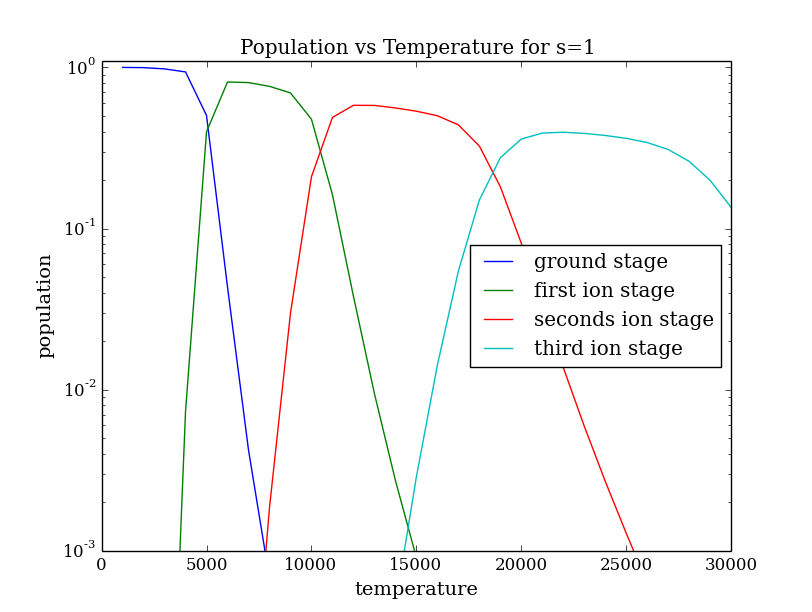
\includegraphics[width=.49\textwidth]{pop_vs_t_for_s1.png}
 \caption{Population as a function of temperature for $s = 1$.}
 \label{pop_vs_t_for_s1}
\end{figure}

Figures for higher levels of s can be seen in figures \ref{pop_vs_t_for_s2} \& \ref{pop_vs_t_for_s4}.
\begin{figure}
 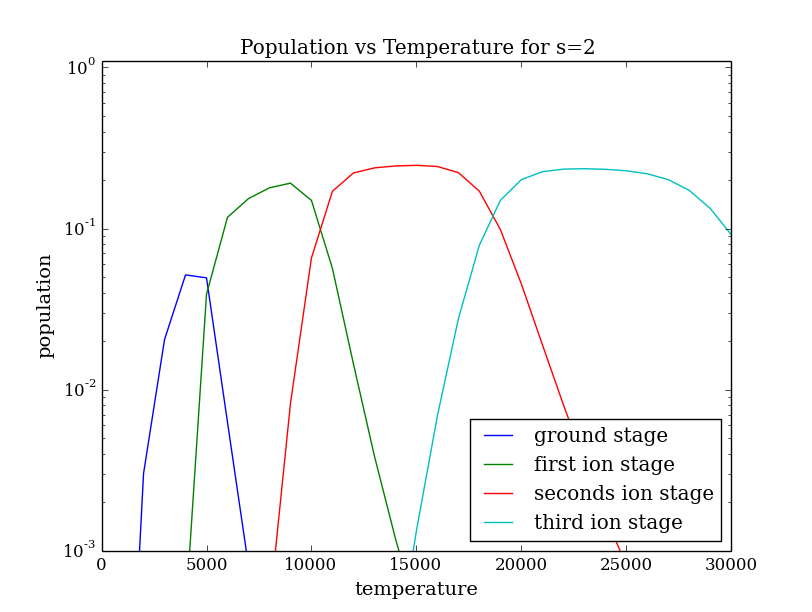
\includegraphics[width=.49\textwidth]{pop_vs_t_for_s2.png}
 \caption{Population as a function of temperature for $s = 4$.}
 \label{pop_vs_t_for_s2}
\end{figure}

\begin{figure}
 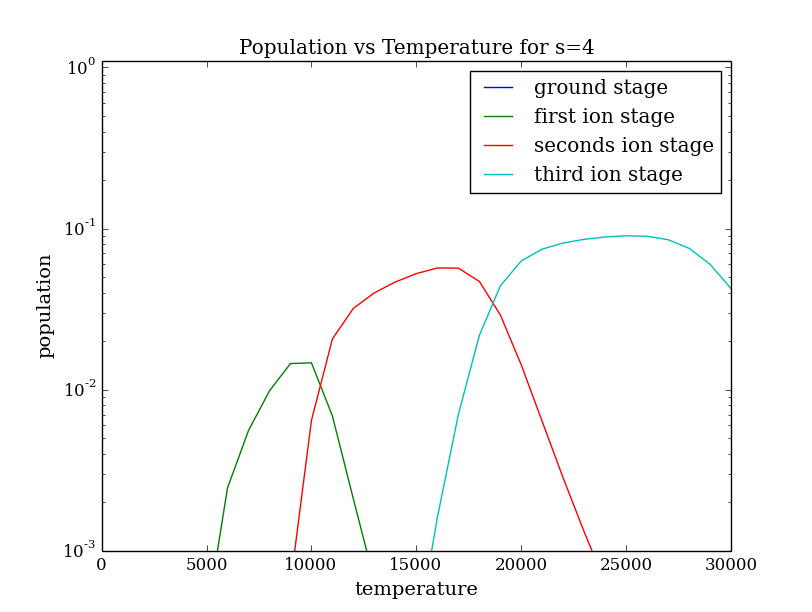
\includegraphics[width=.49\textwidth]{pop_vs_t_for_s4.png}
 \caption{Population as a function of temperature for $s = 4$.}
 \label{pop_vs_t_for_s4}
\end{figure}

The change between the three figures is clear straight away. When looking at the ground state for the energy levels we see that the higher the temperature is, the lower the population gets. Studying the plots for higher energy levels we also see that the population moves to higher energy levels for higher ionization levels. 
If one considers elements with lower ionization energies than E the curves should move towards the right, and become broader. This should become clear by considering the fact that with ionization energies, one would need lower thermal energy to ionize atoms. The edges should be sharper as well, since the fluctuations due to the uncertainty principle can have a bigger impact.
Considering higher ionization energies gives us the opposite case with broader curves moved towards the left and becoming narrower.

\subsection{Saha-Boltzmann population of hydrogen}
Since we've made function for our fictional element it should be easy to transfer this to a real element, namely Hydrogen.
To write the functions for Hydrogen we need to know a few things about it first. Hydrogen has ionization energy $\chi_1 = 13.598$ eV. The statistical weight $g_{r,s}$ and level energies $\chi_{r,s}$ of neutral hydrogen are given by
\begin{equation*}
g_{1,s} = 2s^2 ~,~ \chi_{1,s} = 13.598(1-1/s^2) ~\textmd{eV}
\end{equation*}
while the single ion stage(protons only) has $U_2 = g_{2,1} = 1$.
Implementing this worked nicely and i was able to reproduce the values in the exercise text.
\subsection{Solar Ca$^+$K versus H$\alpha$: line strength}
Studying the spectrum of the sun reveals that the $Ca^+ K$ line is much stronger than the $H\alpha$ line. Even if the ratio between Calcium and hydrogen abundance in the sun is $2*10^6$, and the temperature in the photsphere and chromosphere is $4000-6000$ K, the lower ionization energy for Calcium has the potential to excite many more electrons than the Hydrogen.

To prove this I rewrite the function for Schadeenium and use the ionization energies for Calcium instead. We then plot the ratio between the two lines as a function of temperature. See figure \ref{CaHratio}. Looking at the plot reveals that lower temperature gives higher strength to Calcium. Which makes sense considering the above. As the temperature increases we get enough energy to ionize more and more hydrogen, which makes that stronger than Calcium, since levels 2 and above for Calcium need more energy than the first one for hydrogen. Printing out the ratio at $T = 5000$K gives a ratio of $7643$. This doesn't match the value given in the exercise text perfectly but it is close enough to be considered correct.
\begin{figure}
 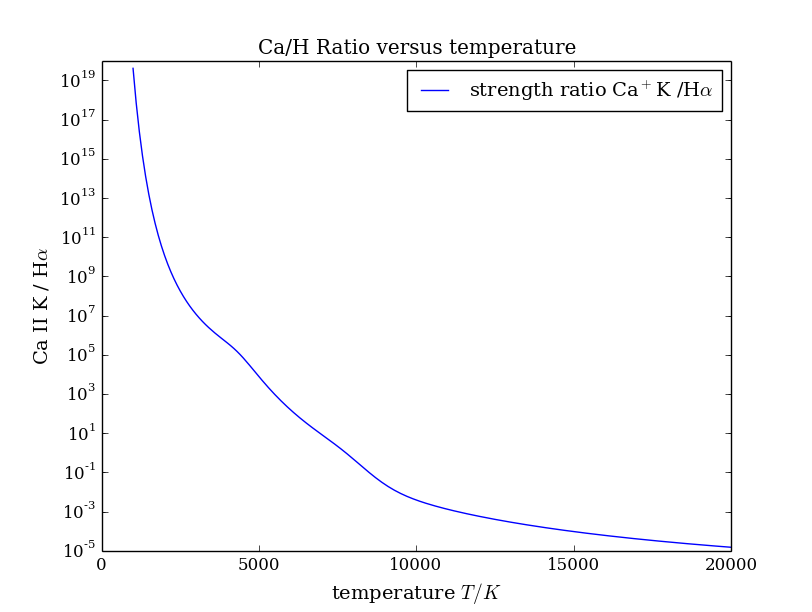
\includegraphics[width=.49\textwidth]{CaHratio.png}
 \caption{Calcium hydrogen ratio as a function of temperature.}
 \label{CaHratio}
\end{figure}

\subsection{Solar Ca$^+$K versus H$\alpha$: temperature sensitivity}
The two lines also differ much in their temperature sensitivity in this formation regime. This can be shown by plotting the relative changes $(\Delta n_{Ca}/\Delta T))/n_{Ca}$ and $(\Delta n_H/n_H)$ for the two lower levels as function of temperature for a small change in temperature $\Delta T$. See figure \ref{relpopchange} for a plot of this. Studying the plot we see two dips, one for Ca$^+$K around $T = 5600$K, and one for H$\alpha$ around $T = 9500$K. From this we can also see that the left side of each dip has $\Delta n < 0$, while the right side has $\Delta n > 0$. To take a closer look at the dips we plot the variation with temperature of each population in relative units on top of the last figure, resulting in figure \ref{relpopchange2}. We see that the relative population for Calcium starts increasing from the start which we expect from its lower ionization energy. After a while all of the Calcium is ionized, and after a bit more we start ionizing the next level and thus the population of this level starts falling. The same mechanism works on hydrogen, but it doesnt fall as fast because of its higher ionization energy. From this it is clear that since the populations remain almost constant for some range of temperatures, the change in the population has to shrink drastically during this range, and that is exactly what we're seeing in the plot. (The dips are right below the tops of the other curves.)
\begin{figure}
 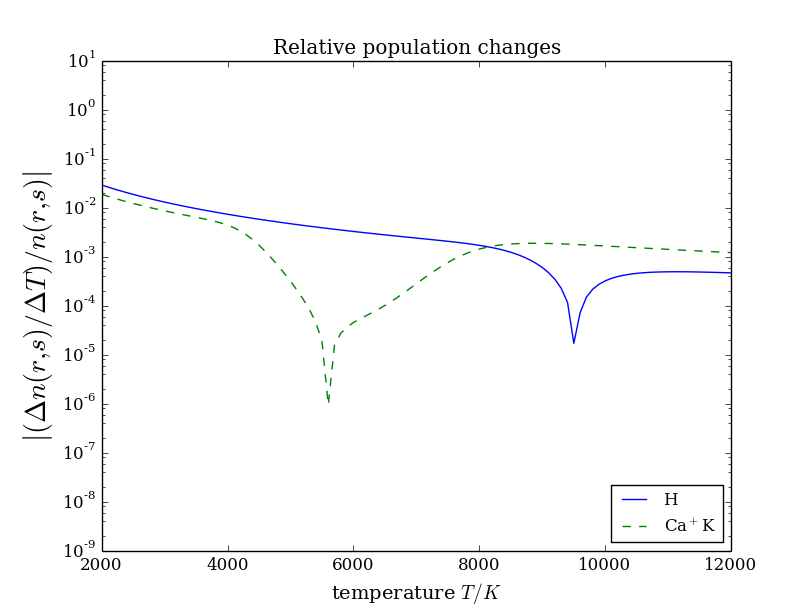
\includegraphics[width=.49\textwidth]{relpopchange.png}
 \caption{Relative population change vs temperature.}
 \label{relpopchange}
\end{figure}
\begin{figure}
 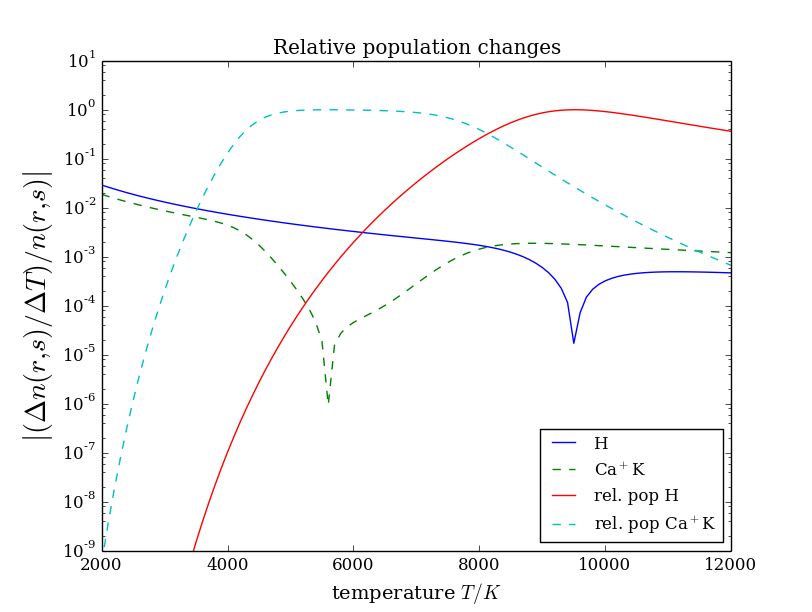
\includegraphics[width=.49\textwidth]{relpopchange2.png}
 \caption{Relative population change vs temperature in relative units.}
 \label{relpopchange2}
\end{figure}

\subsection{Hot stars versus cool stars}
Finally for this section we want to know what temperature corresponds to about $50\%$ ionization for stellar photospheres with $P_e = 10^2$. To find this we plot the neutral hydrogen fraction versus temperature and get figure \ref{hydrogen_ionization}, where it looks to be about $9200 K$.
\begin{figure}
 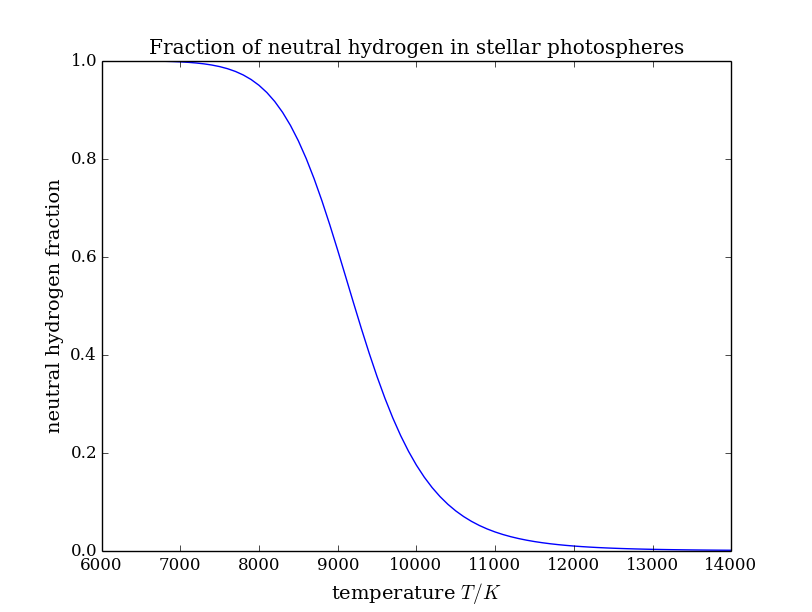
\includegraphics[width=.49\textwidth]{hydrogen_ionization.png}
 \caption{Neutral hydrogen fraction versus temperature.}
 \label{hydrogen_ionization}
\end{figure}
%%%%%%%%%%%%%%%%%%%%%%%%%%%%%%%%%%%%%%%%%%%%%%%%%%%%%%%%%%%%%%%%%%%%%%%%%%%%
\section{Fraunhofer line strengths and the curve of growth}   \label{sec:Fraunhofer}
%%%%%%%%%%%%%%%%%%%%%%%%%%%%%%%%%%%%%%%%%%%%%%%%%%%%%%%%%%%%%%%%%%%%%%%%%%%%
\subsection{The Planck law}
The Planck law is the counterpart to the Saha and Boltzmann distributions for radiation. It specifies the radiation intensity emitted by a gas or body in thermal equilibrium. This is known as a black body. The function is defined
\begin{equation}
 B_\lambda(T) = \frac{2hc^2}{\lambda^5}\frac{1}{e^{hc/\lambda kT}-1}
\end{equation}\label{Planck}

We plot this for the visible spectrum for some temperatures in figure \ref{radiation}. We see that the top shifts to lower wavelengths for higher temperatures. We also see that the left side follows the Wien approximation, while the right side follow the Rayleigh-Jeans approximation.
\begin{figure}
 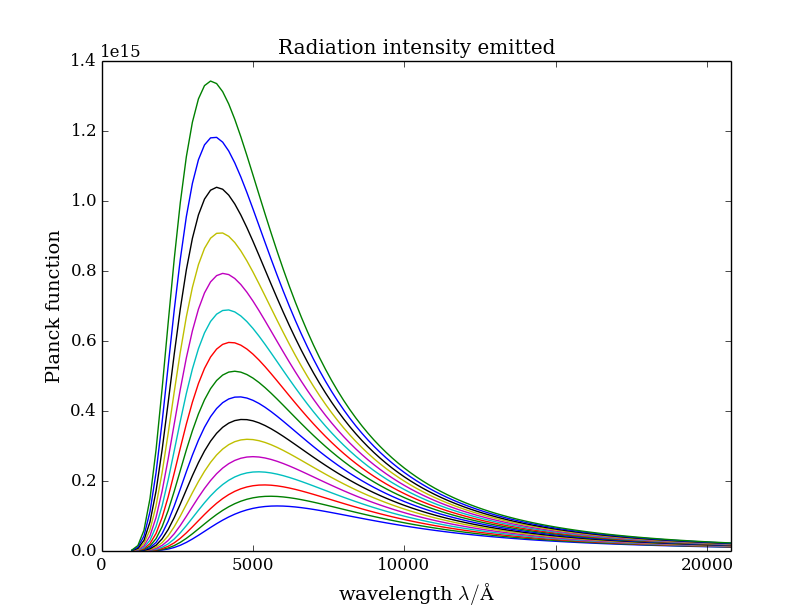
\includegraphics[width=.49\textwidth]{radiation.png}
 \caption{Planck function for the visible spectrum using different temperatures.}
 \label{radiation}
\end{figure}
The same plot with a logarthmic scale on the y axis can be seen in figure \ref{radiation_ylog}, and the same plot with both axes logarithmic can be seen in figure \ref{radiation_ylog_xlog}. Here we can see even clearer that the Rayleigh-Jeans approximation is correct.
\begin{figure}
 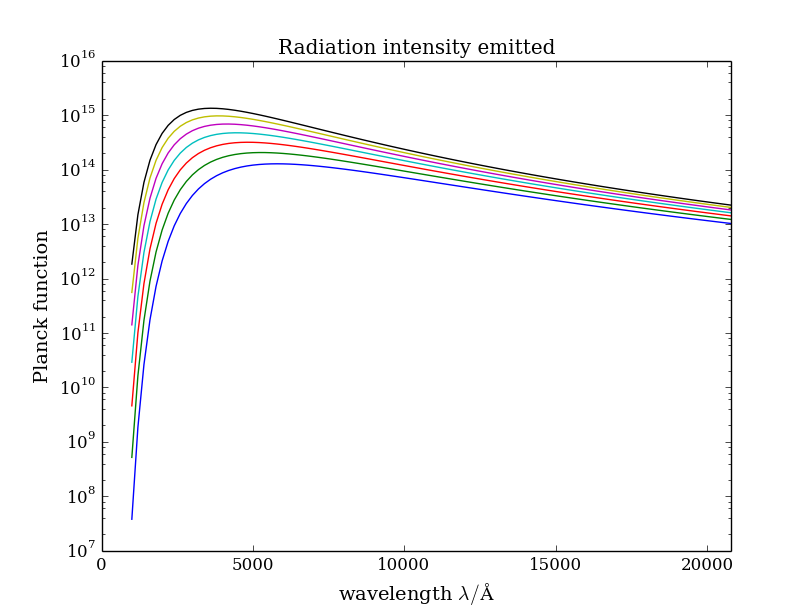
\includegraphics[width=.49\textwidth]{radiation_ylog.png}
 \caption{Logarthimic y axis.}
 \label{radiation_ylog}
\end{figure}
\begin{figure}
 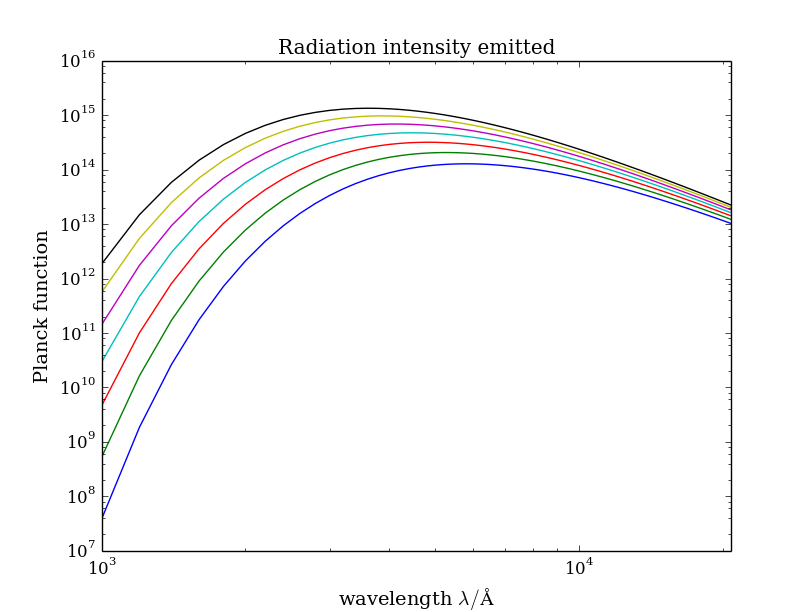
\includegraphics[width=.49\textwidth]{radiation_ylog_xlog.png}
 \caption{Both axes logarithmic.}
 \label{radiation_ylog_xlog}
\end{figure}

\subsection{Radiation through an isothermal layer}
It can be shown that the total emergent radiation from a layer with optical thickness $\tau(x)$ and temperature $T(x)$ is:
\begin{equation}\label{Radiation_general}
\begin{aligned}
 I_{\lambda} =& I_{\lambda}(0)e^{-\tau} + \int_0^\tau B_{\lambda}[T(x)]e^{-(\tau - \tau(x))}d\tau(x)
\end{aligned}
\end{equation}
If one assumes that the layer is isothermal, this implies that the optical thickness and temperature is independent of position inside the layer. Inserting this into equation \ref{Radiation_general} gives the following

\begin{equation*}
\begin{aligned}
I_{\lambda} =& I_{\lambda}(0)e^{-\tau} + \int_0^\tau B_{\lambda}[T(x)]e^{-(\tau - \tau(x)')}d\tau(x)'\\
	    =& I_{\lambda}(0)e^{-\tau} + B_{\lambda}(T)e^{-\tau}\int_0^\tau e^{\tau'}d\tau'\\
	    =& I_{\lambda}(0)e^{-\tau} + B_{\lambda}(T)e^{-\tau}(e^{\tau} - 1)\\
\end{aligned}
\end{equation*}

\begin{equation}\label{Radiation_isothermal}
 I_{\lambda} = I_{\lambda}(0)e^{-\tau} + B_{\lambda}(1 - e^{-\tau})
\end{equation}
Now if we plot this function for $\tau = [0.01,10]$ with $B = 2$, and $I_{\lambda}(0) = [0,4]$ we get figure \ref{emergent_original}, and if we make the axes logarthimic we get figure \ref{emergent_log}.

\begin{figure}
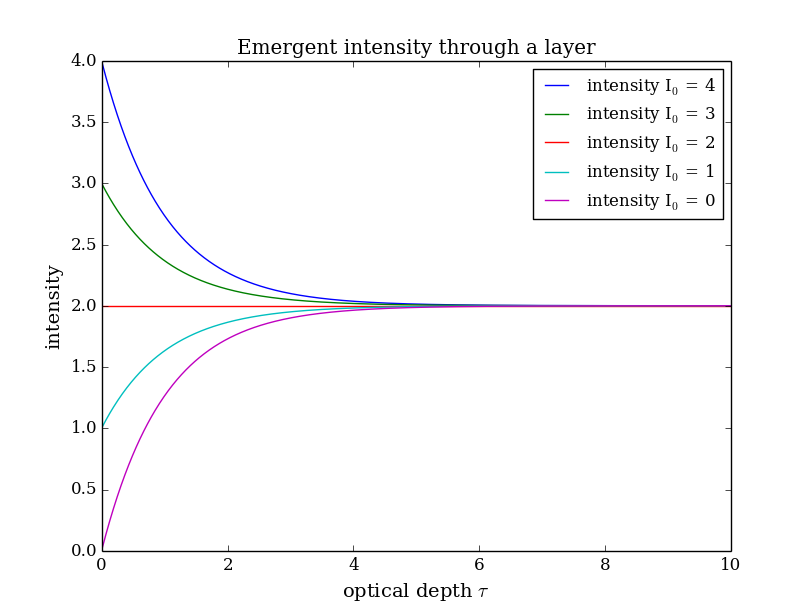
\includegraphics[width=.49\textwidth]{emergent_original.png}
\caption{As the optical depth increases, the intensity converges to the intensity of the Source function B.}
\label{emergent_original}
\end{figure}

\begin{figure}
 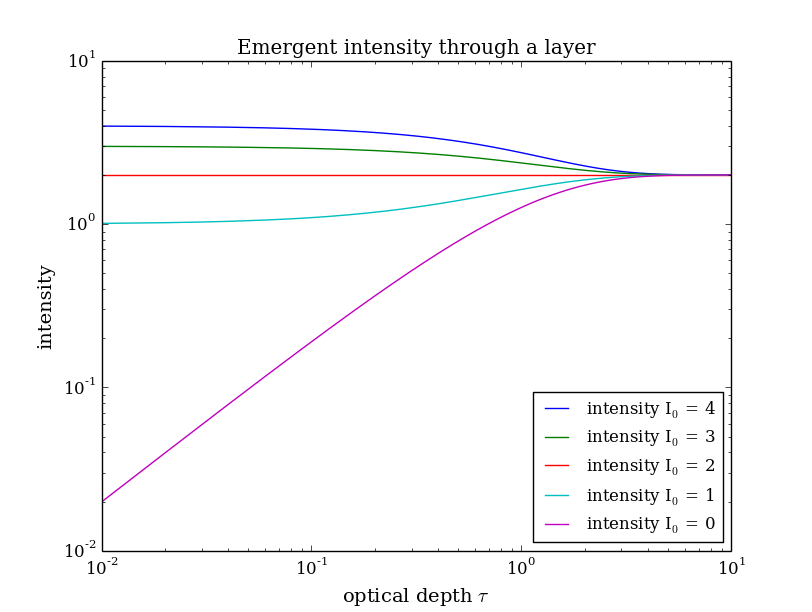
\includegraphics[width=.49\textwidth]{emergent_log.png}
 \caption{The emergent intensity with a logarthimic scale.}
 \label{emergent_log}
\end{figure}
Studying figures \ref{emergent_original} \& \ref{emergent_log} shows a few different things.
If one first considers cases where $\tau << 1$, the figures show that if $I_\lambda(0) = 0$, you get an exponential growth due to the source function B. And if $I_\lambda(0) > B_\lambda$ the intensity stays close to constant. This case corresponds to an ``optically thin'' medium. This is because whatever intensity that enters the medium passes straight through without being affected by the medium.

The opposite case where $\tau >> 1$ is called an ``optically'' thick medium, since all the incident radiation is absorbed before it is able to pass through, and is replaced by the radiation emitted by the medium itself. As seen in the plot, the emergent intensity becomes independent of optical depth for large $\tau$. Mathematically this can be seen by looking at equation \ref{Radiation_isothermal} and letting $\tau \rightarrow \infty$. In physical terms one can picture it such that both the incident radiation and the radiation emitted by the medium is absorbed while it is passing through the medium, but since the medium replenishes the radiation it is emitting along the path through it, this radiation is refilled as one goes through the medium,while the incident radiation ``runs out'' after some distance.

From this it should be clear that optically thin mediums allow us to view radiation originating from the other side of the medium, while optically thick mediums absorb all of the incident radiation before it can pass through, thus blocking our view past them.

\subsection{Spectral lines from a solar reversing layer}
At this point we choose to use the Schuster-Schwarzschild model. Another name for this model is a reversing-layer model.
This model works on the assumption that the continous radiation, without spectral lines, is emitted by the surface of the star, and this radiation then irradiates a seperate layer around the star.
This layer is then hit by an intensity
\begin{equation}
 I_\lambda(0) = B_\lambda(T_{surface}).
\end{equation}\label{Surface layer}
This causes emission only at the wavelengths of spectral lines. 
Next, ones assumes that the star is optically thick, so that the surfrace radiates with the solution of equation \ref{Radiation_isothermal} where $\tau << 1$, meaning $I_\lambda = B_\lambda(T_{surface})$. This does not mean that shell has to be optically thick. The line-causing atoms in the shell have their own temperature $T_{layer}$, giving a local production of radiation in the layer for the line-wavelength $B_\lambda(T_{layer})\Delta\tau(x)$. Combining equation \ref{Radiation_isothermal} \& \ref{Reversing layer} yields
\begin{equation}
 I_\lambda =B_\lambda(T_{surface})e^{-\tau_\lambda} + B_\lambda(T_{layer})(1 - e^{-\tau_\lambda})
\end{equation}\label{Reversing layer}
Note that the opaqueness $\tau$ in equation \ref{Reversing layer} has gotten an index for wavelength, since it depends on wavelength.

\subsubsection{Voigt function}
In reality spectral lines are not infinitely sharp delta functions. This can be attributed to Doppler shifts and Coloumb interactions between neighbouring particles. (Even if one could get rid of those effects, you would still have the uncertainty principle spreading it out a little.)

This broadening of the spectral line is described by the distribution
\begin{equation}
 \tau(u) = \tau(0)V(a,u)
\end{equation}\label{distribution}
where V is the Voigt function, and u describes the the wavelength separation from the center of the line such that
\begin{equation}
 u \equiv \Delta\lambda/\Delta\lambda_D
\end{equation}
where
\begin{equation}
 \Delta\lambda_D \equiv \frac{\lambda}{c} \sqrt{2kT/m}.
\end{equation}
Here m is the mass of the line-causing particles.
The $a$ parameter measures the Coloumb disturbances. For stellar atomspheres $a$ is usually somewhere in the range $[0.01,0.5]$. The definition of the Voigt function is
\begin{equation}
 V(a,u) = \frac{1}{\Delta\lambda_D\sqrt{\pi}}\frac{a}{\pi}\int_{-\infty}^{+\infty}\frac{e^{-y^2}}{(u-y)^2 + a^2}dy
\end{equation}\label{Voigt}
The Voigt profile represents the convolution(smearing) of a Gauss profile using a Lorentz profile. Because of this it has a Gaussian shape close to line center, and Lorentzian wings on the edges.
This can be approximated by taking the sum instead of the convolution giving 
\begin{equation}
 V(a,u) = \frac{1}{\Delta\lambda_D\sqrt{\pi}} \bigg[e^{-u^2} + \frac{a}{\sqrt{\pi}u^2}\bigg]
\end{equation}\label{Voigt_approx}

For those using IDL to do calculations, the Voigt function is ready for use through the appropriately named function voigt.
Since I use python we instead have to use the fact that the voigt function can be written
\begin{equation}
 V(x;\sigma,\gamma) = \frac{Re[w(z)]}{\sigma \sqrt{2\pi}}
\end{equation}
where Re[w(z)] is the real part of the Faddeeva function evaluated for 
\[
 z = \frac{x + i\gamma}{\sqrt{2}\sigma} ~,~ a = \frac{\sigma}{\sqrt{2}\sigma} ~,~ u = \frac{x}{\sqrt{2}\sigma}.
\]
In this case the factor $\Delta\lambda_D = \sqrt{2}\sigma$.
Luckily for us the Faddeeva function can be found in the special module of the scipy package for python, so that is what we will be using. If we plot this function for different values of $a$ for $u = [-10, 10]$ we get figure \ref{voigt_orig}.
\begin{figure}
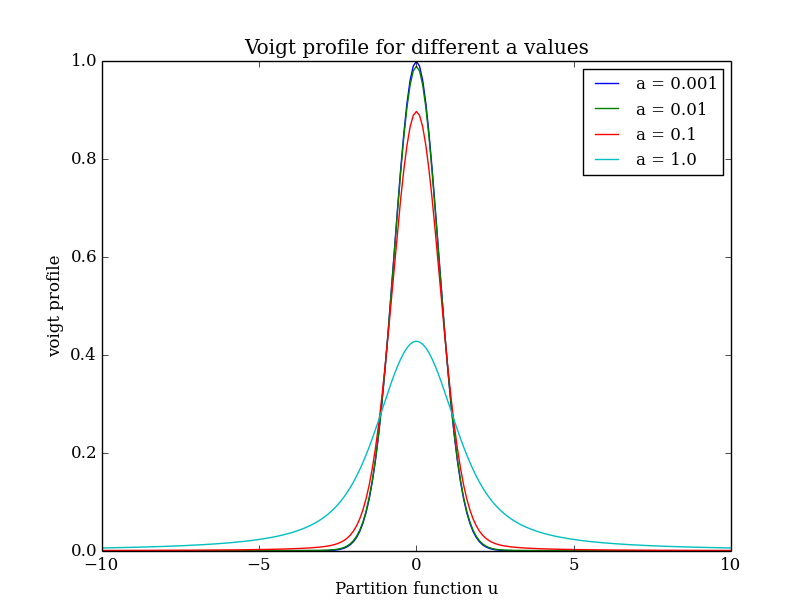
\includegraphics[width=.49\textwidth]{voigt_original.png}
\caption{Voigt profile for different values of a.}
\label{voigt_orig}
\end{figure}
To study this we plot the same, but this time with a logarthimic scale for the y axis. The plot can be seen in figure \ref{voigt_ylog}.
\begin{figure}
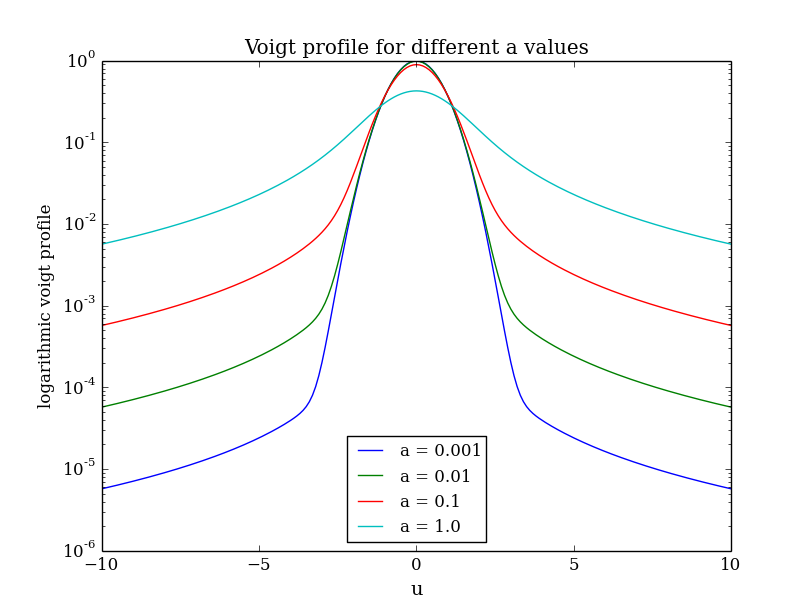
\includegraphics[width=.49\textwidth]{voigt_ylog.png}
\caption{Logarithmic voigt profile for different values of a.}
\label{voigt_ylog}
\end{figure}
Using approximation \ref{Voigt_approx} it is clear that the the exponential term vanishes very quickly as $|u|$ increases, leaving us with
\[
 V(a,u) \approx \frac{a}{\Delta\lambda_D\pi u^2} 
\]
which gives the functions the same form on the wings just scaled by the factor $a$.

\subsubsection{Emergent line profiles}
We now have both functions for intensity and for the distribution of the optical depth. By combining equation \ref{Radiation_isothermal} \& \ref{distribution} we should be able to compute and plot stellar spectral line profiles!
To do this we use values that fit well with the solar photosphere and plot what it looks like in the visible spectrum.
The values we will be using are $T_{surface} = 5700 K$, $T_{layer} = 4200 K$, $a = 0.01$, $\lambda = 5000 \AA$.
We start by plotting the intensity against $u$ for $\tau(0) = 1$. This results in figure \ref{emergent_line_orig_5000}.
\begin{figure}
 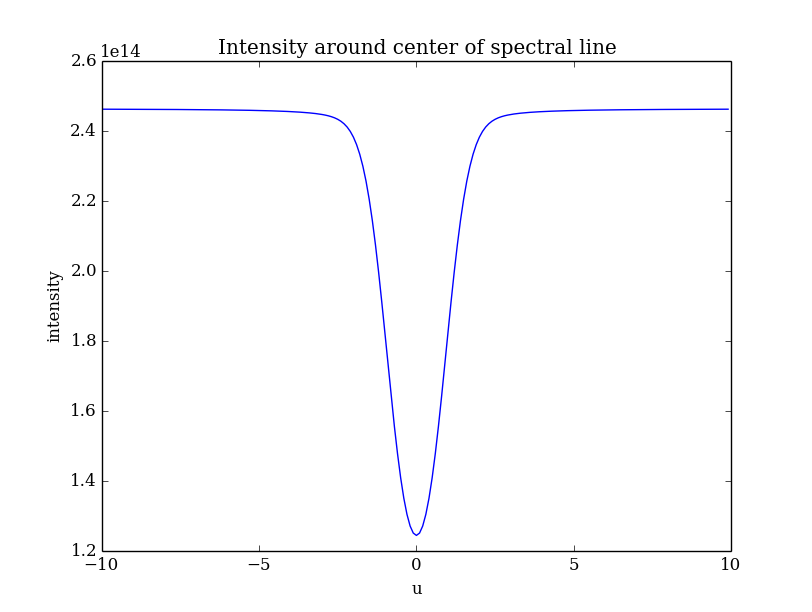
\includegraphics[width=.49\textwidth]{emergent_line_orig_5000.png}
 \caption{Spectral lines for wavelength $5000 ~\AA$.}
 \label{emergent_line_orig_5000}
\end{figure}

Next we study the behaviour of the line for $\tau(0)$ in the range $\log \tau(0) = [-2, 2]$.
This results in figure \ref{emergent_line_log_5000}. Studying this plot reveals that $\tau(0)<<1$ lose almost none of their intensity, just as expected for optically thin media. We also see the ``refilling'' behaviour of the source function which keeps the saturation above a minimum level. Note also the line wiwngs developing for large $\tau(0)$. This can be attributed to the fact that the intensity is dependent on $\tau$ which is dependent on $\tau(0)$ and $V(a,u)$. So the larger $\tau(0)$ is, the longer the exponential terms in equation \ref{Reversing layer} can reduce the intensity. In fact these ``wings'' don't really converge to the continuum until $u \rightarrow \pm \infty$. We can also see from this plot wether the medium is optically thin or thick by recalling that we separate the domains of thickness at the point where the emergent radiation has been reduced to a factor $1/e$ of its incident radiation. In this case we see from the plot that the incident radiation is about $2.5\times 10^{14}$ so anything below about $0.9\times 10^14$ is optically thick, while anything above is optically thin.
Thus we see that from the plot that in this case we get an optically thick medium if $\log \tau(0)= 0$ or less. Strictly
speaking the limit is somwhere between this and $\log \tau(0) = 0.5$. If we shift our view to the sides of the line center to e.g $ u = 5$ all of the plotted lines are well above the limit for optically thin.
\begin{figure}
 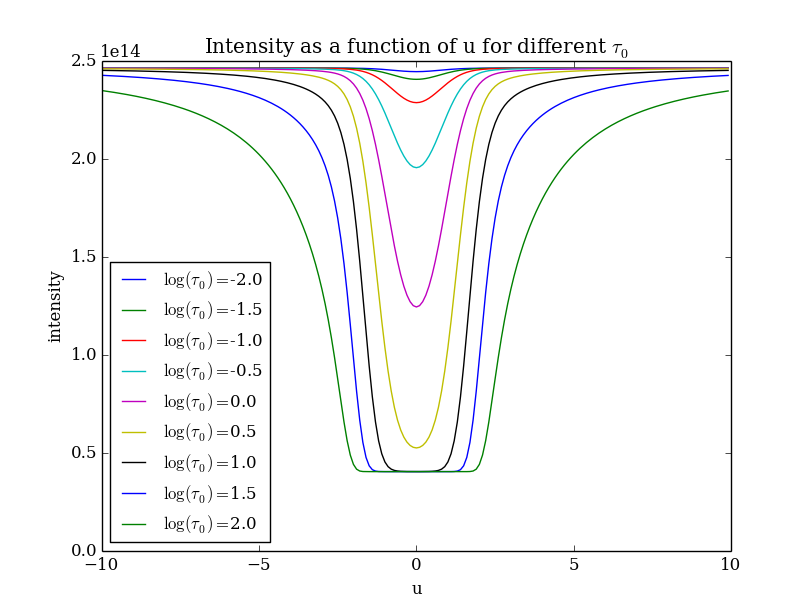
\includegraphics[width=.49\textwidth]{emergent_line_log_5000.png}
 \caption{Spectral lines for different choices of $\tau(0)$ at $\lambda = 5000 \AA$.}
 \label{emergent_line_log_5000} 
\end{figure}

Looking at the spectral lines for different wavelengths reveal a difference in intensity. This can be seen in figure \ref{emergent_line_orig}.
To check the behaviour for different wavelengths we plot the results for $\lambda = 2000$ \& $10000$ in figures  \ref{emergent_line_log_2000} $\&$ \ref{emergent_line_log_10000}.

\begin{figure}
 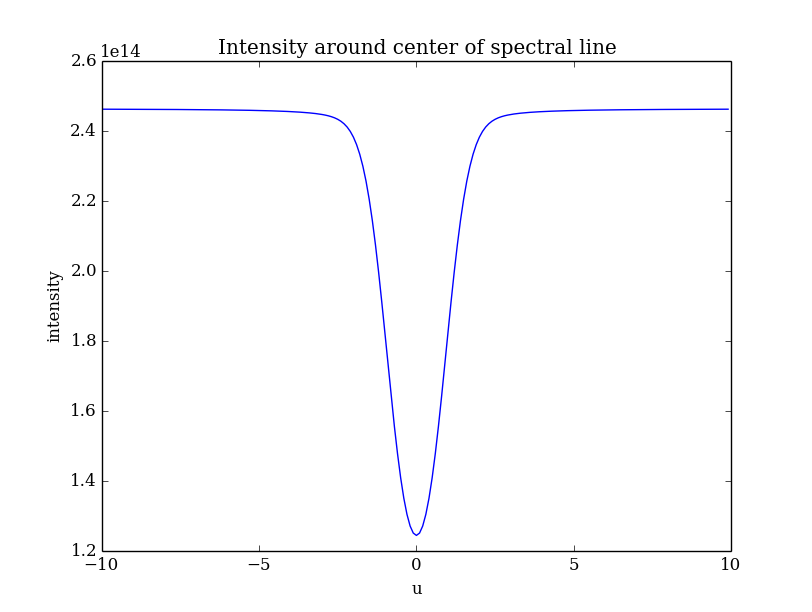
\includegraphics[width=.49\textwidth]{emergent_line_orig.png}
 \caption{Spectral lines for different wavelengths.}
 \label{emergent_line_orig}
\end{figure}
\begin{figure}
 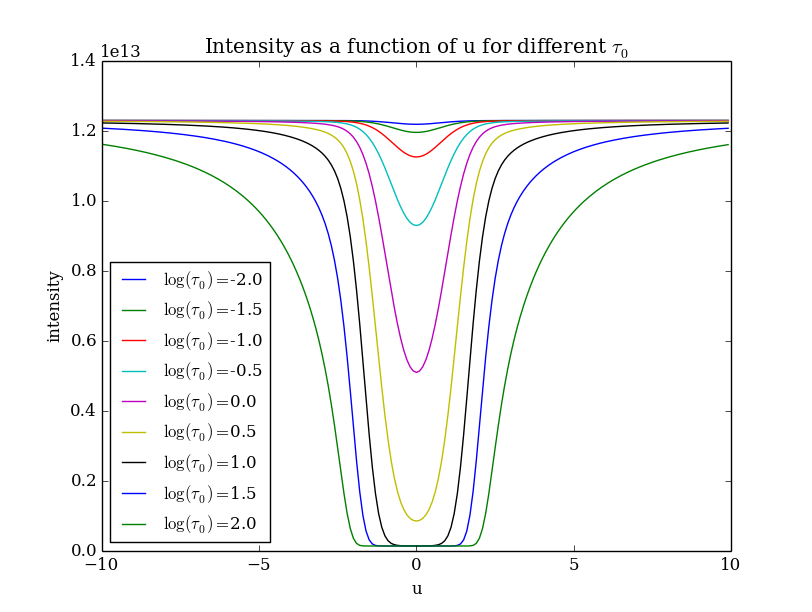
\includegraphics[width=.49\textwidth]{emergent_line_log_2000.png}
 \caption{Spectral lines for different choices of $\tau(0)$ at $\lambda = 2000 \AA$.}
 \label{emergent_line_log_2000} 
\end{figure}
\begin{figure}
 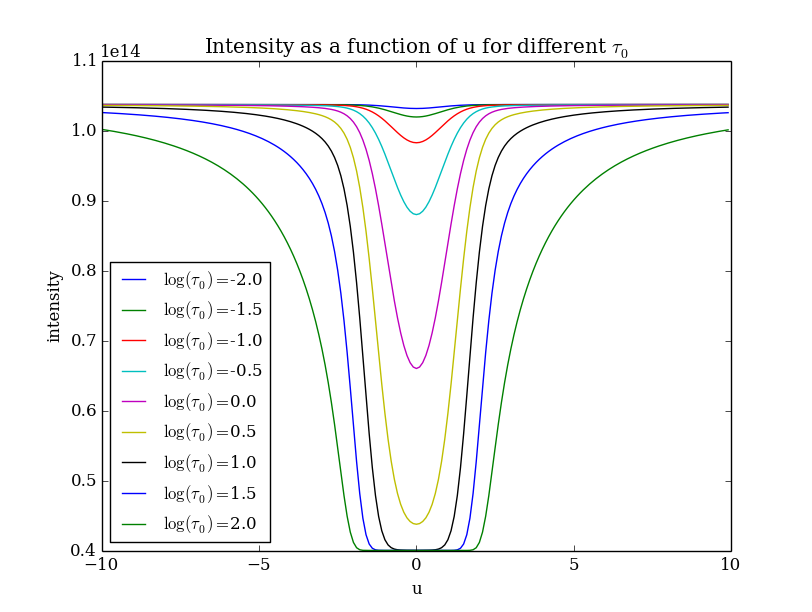
\includegraphics[width=.49\textwidth]{emergent_line_log_10000.png}
 \caption{Spectral lines for different choices of $\tau(0)$ at $\lambda = 10000 \AA$.}
 \label{emergent_line_log_10000} 
\end{figure}

For the two other wavelengths we see the same behaviour as we did for $\lambda = 5000 \AA$. The shapes are the same, while the intensity of the continuum changes. The lower limit also moves. For $\lambda = 2000 \AA$ we end up with a separation between optically thin and thick at roughly the same place as for $\lambda = 5000 \AA$. However, for $\lambda = 10000 \AA$ the intensity reaches the lower limit before it can be reduced to the point where we say the medium is optically thick. This would indicate that the medium is optically thin at very high wavelengths. To find the value of the continuum we look at the equation for the emergent intensity (eq. \ref{Reversing layer}). To look at the continuum we set $\tau \rightarrow 0$, since the continuum should have no optical depth. This gives 
\begin{equation}
I_{cont}  = B_\lambda(T_{surface})
\end{equation}
so the intensity of the continuum is defined by the surface temperature.
While if we let $\tau \rightarrow \infty$ we get the lower limit
\begin{equation}
I_{min}  = B_\lambda(T_{layer})
\end{equation}
We check these values by printing them to the commandline in our function. The results of this can be found in table \ref{I_Cont}. Calculating them from the Planck function gives the same answers.
\begin{table}
\begin{center}
\begin{tabular}{| c | c | c |}
\hline
$\lambda$ & $I_{cont}$ & $I_{center}$\\
\hline
2000 & $1.23\times 10^{13}$ & $1.36\times 10^{11}$\\
\hline
5000 & $2.46\times 10^{14}$ & $4.04\times 10^{13}$\\
\hline
10000 & $1.04\times 10^{14}$ & $4.00\times 10^{13}$\\
\hline
\end{tabular}\label{I_Cont}
\caption{Intensity of the continuum}
\end{center}
\end{table}
Since some observed spectra are measured without absolute intensity calibration it is useful to scale the spectrum to the local continuum intensity by plotting $I_\lambda/I_{cont}$. Plotting this for the same 3 wavelengths reults in figure \ref{emergent_line_scaled_different}.
\begin{figure}[hbtp]
 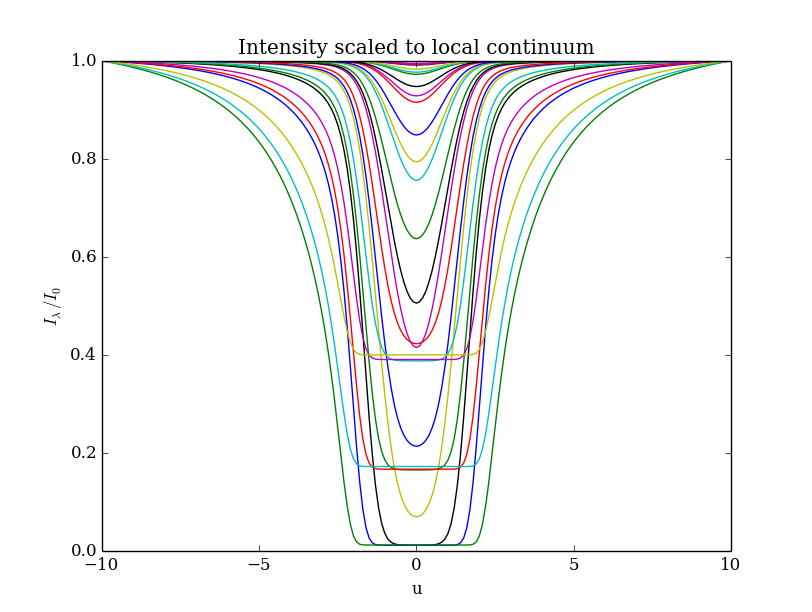
\includegraphics[width=.49\textwidth]{emergent_line_scaled_different.png}
 \caption{Spectral lines for different choices of $\tau(0)$.}
 \label{emergent_line_scaled_different} 
\end{figure}
Here we see clearly that the wavelength of the radiation is crucial to whether or not the medium is optically thin or thick.
\subsection{The equivalent width of spectral lines}
From the profile plots one can see that the growth of the absorption feature for increasing $\tau(0)$is faster for small $\tau(0)$ than for larger $\tau(0)$. Because of this, Minnaert and his coworkers introduced the equivalent width $W_\lambda$ as a line-strength parameter to measure this effect. It measures the integrated line depression in the normalized spectrum
\begin{equation}
 W_\lambda = \int \frac{I_{cont}-I(\lambda)}{I_{cont}}d\lambda.
\end{equation}\label{eqw}
To test this effectively we make a profile function that returns a Schuster-Schwarzschild profile, given $a$, $\tau$, and $u$.  Setting $a = 0.1$, $\tau(0) = 100$ and plotting this for $ u = [-200,200]$ returns figure \ref{eqw_ss}.
\begin{figure}
 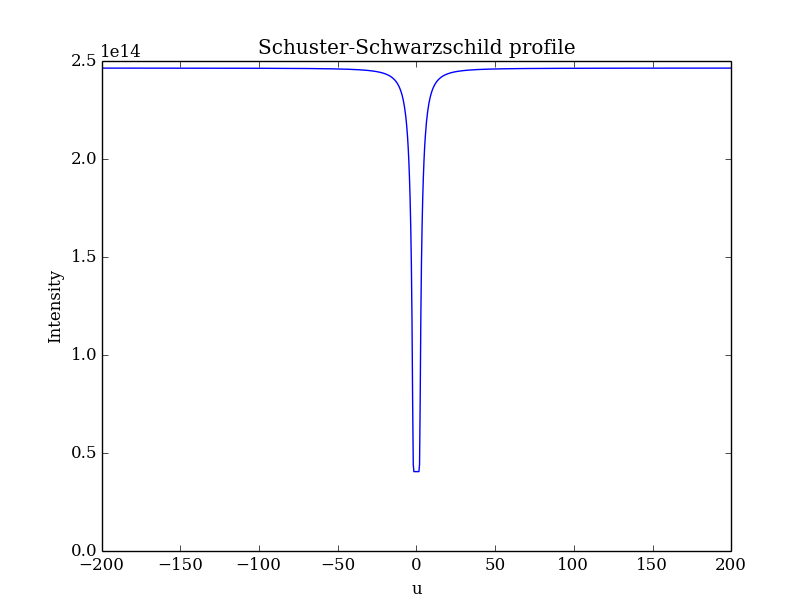
\includegraphics[width=.49\textwidth]{eqw_ss.png}
 \caption{Schuster-Schwarzschild profile.}
 \label{eqw_ss} 
\end{figure}

Next we compute the line depth in relative units(the integrand in equation \ref{eqw}. Plotting this versus u gives figure \ref{eqw_rel}.
\begin{figure}
 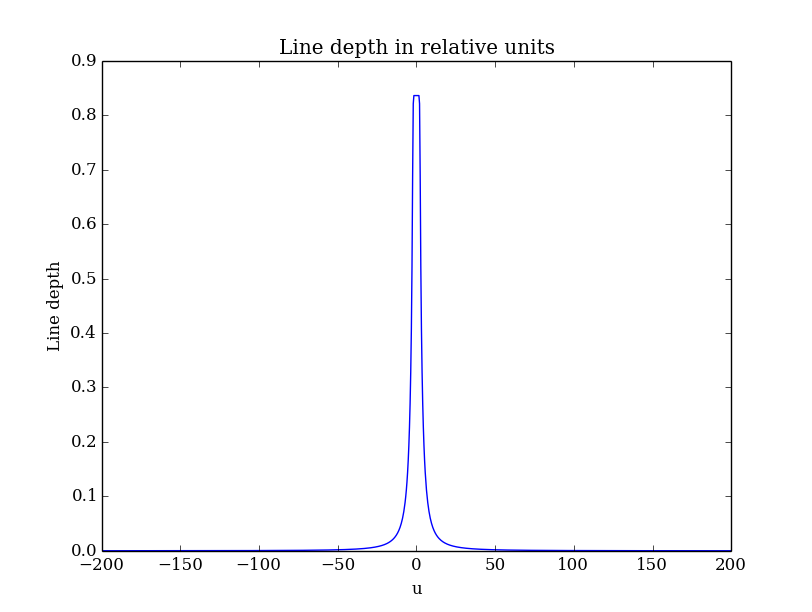
\includegraphics[width=.49\textwidth]{eqw_rel.png}
 \caption{Line depth in relative units.}
 \label{eqw_rel} 
\end{figure}

In this test case we get an equivalent width $W_\lambda = 7.5$.

\subsection{The curve of growth}
The point of the equivalent width was that it could be used to measure the number of atoms in the reversing layer. This should set the opaqueness $\tau(0)$ of the layer. The profile plots show that the profile growth is only linear with $\tau(0)$ for $\tau(0) <<1$. The curve of growth shows the full dependence; the growth of the line strength with the line-causing density.
To study this we plot $\log W_\lambda$ against $\log \tau(0)$ in figure \ref{growth}.
\begin{figure}
 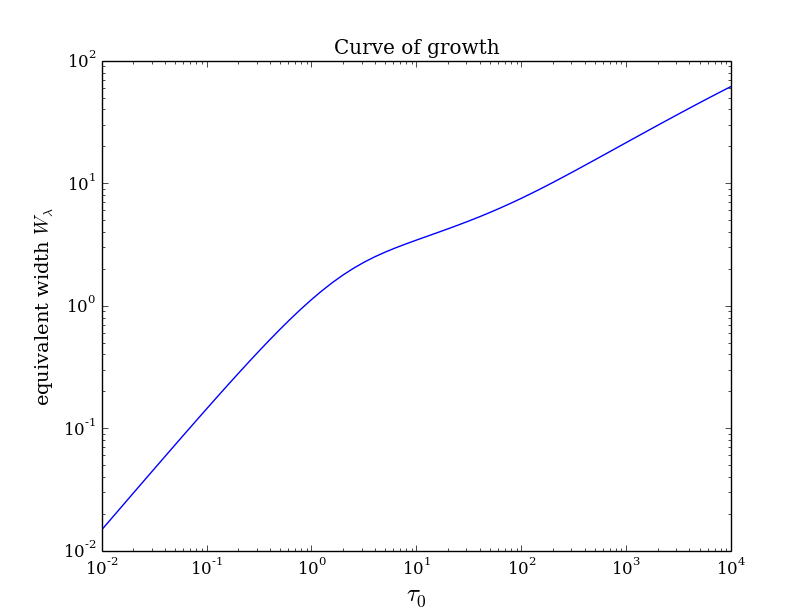
\includegraphics[width=.49\textwidth]{growth.png}
 \caption{Curve of Growth.}
 \label{growth} 
\end{figure}
Studying the curve of growth is easier if we also look at the corresponding emergent line profiles(see fig. \ref{emergent_line_log_5000}.) For the first part of the growth curve has slope 1:1, here we are in the $\tau << 1$ regime, and we see the emission growth curves becoming larer and larger gauss curves. This continues until we reach the minimum saturation limit where $\tau \approx 1$, where the growth stagnates. This we see in the growth curve in the middle part. After a while we enter the $\tau >> 1$ regime, where the wings of the spectral lines start developing, and thus the slop of the growth function increases as well. However, the growth isn't as rapid here as it was for the $\tau << 1$ regime so we only get a slope of 1:2.
To change the onset of the last part we can change the Couloumb damping parameter $a$. Running the calculation again with $a = 10$ proves this, as can be seen in figure \ref{growth_a10}. Since it is clear that this parameter controls the growth curve, we can use it to estimate its value for solar ironlines by comparing the curves we get from the program to figure 14 in the exercise text. Numerous tests with different $a$ values puts it somewhere in the range $a = [0.01, 0.1]$.
\begin{figure}
 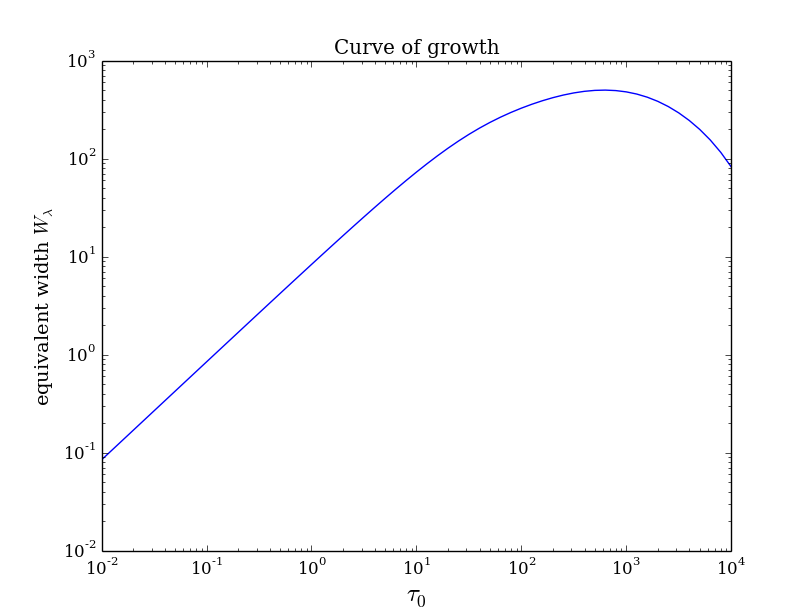
\includegraphics[width=.49\textwidth]{growth_a10.png}
 \caption{Curve of Growth with $a = 10$.}
 \label{growth_a10} 
\end{figure}
So far we've only looked at absorption lines. To produce emission lines we need to change either the temperature of the surface or the temperature of the reversing layer. I choose to change the temperature of the reversing layer to $T_{layer} = 9200$K. Plotting the lines for $\lambda = 5000 \AA$ results in figure \ref{emission5000}.And if we also plot the growth curve for this setup we get figure \ref{emission_growth}. We see that the growth curves look nearly identical, which is expected since the curves are almost mirror images of each other for the spectral lines.
\begin{figure}
 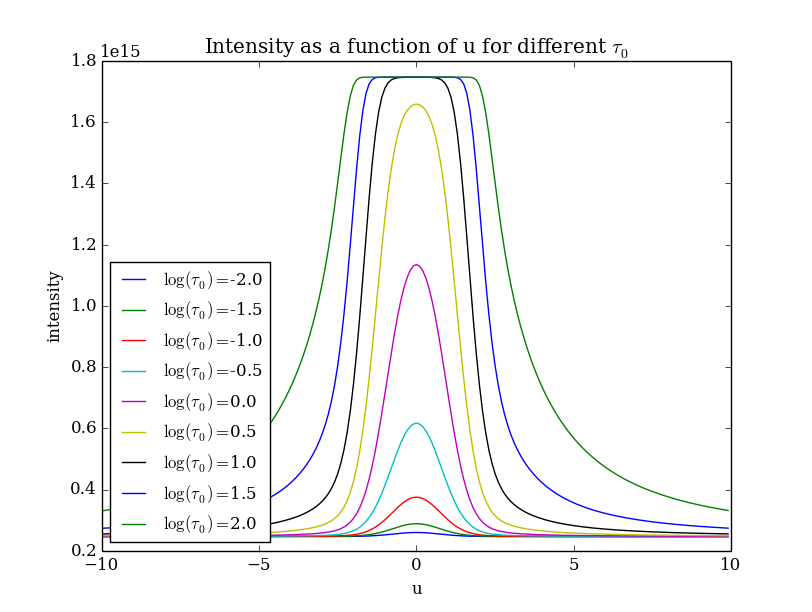
\includegraphics[width=.49\textwidth]{emission5000.png}
 \caption{Emission lines at $\lambda = 5000 \AA$.}
 \label{emission5000} 
\end{figure}
\begin{figure}
 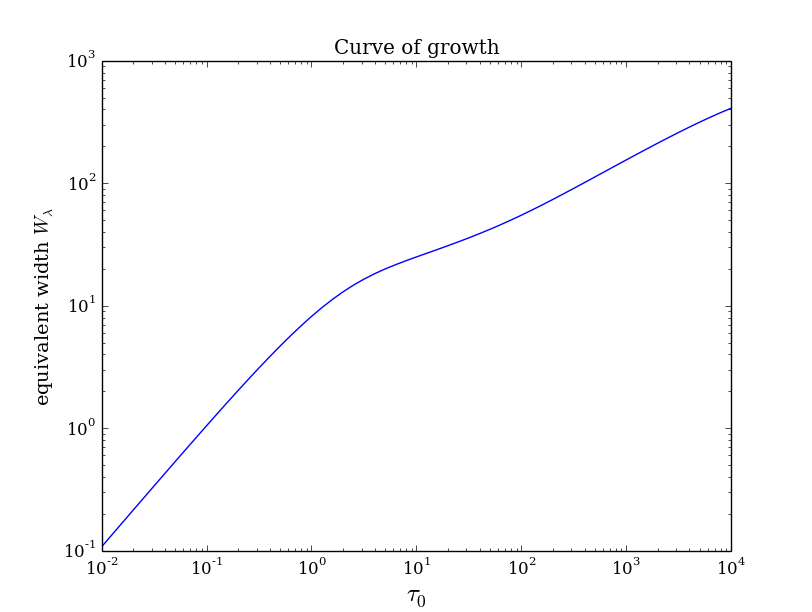
\includegraphics[width=.49\textwidth]{emission_growth.png}
 \caption{Growth curve for emission lines.}
 \label{emission_growth} 
\end{figure}

%%%%%%%%%%%%%%%%%%%%%%%%%%%%%%%%%%%%%%%%%%%%%%%%%%%%%%%%%%%%%%%%%%%%%%%%%%%%
\section{Conclusions} \label{sec:conclusions}
%%%%%%%%%%%%%%%%%%%%%%%%%%%%%%%%%%%%%%%%%%%%%%%%%%%%%%%%%%%%%%%%%%%%%%%%%%%%
In this project we've seen how the Saha and Boltzmann distributions control the ionization and energy levels of elements. We tried using this to study Ca$^+$K and H$\alpha$ lines. We saw that even though there is a lot less Calcium in the sun, the Ca$^+$K lines was much stronger because of its lower ionization energy.
We also saw how the Planck function in combination with the Voigt profile can be used to model spectral lines. This was achieved by using a reversing layer model, where the temperatures of the surface of the sun and the reversing layer controlled whether or not we got absorption or emission lines. With this we were also able to create growth curves, which in turn could be used to approximate the Coloumb damping parameter for solar iron lines by comparing with measurements.
%%%%%%%%%%%%%%%%%%%%%%%%%%%%%%%%%%%%%%%%%%%%%%%%%%%%%%%%%%%%%%%%%%%%%%%%%%%%
%\begin{acknowledgements}
%\end{acknowledgements}

%%%%%%%%%%%%%%%%%%%%%%%%%%%%%%%%%%%%%%%%%%%%%%%%%%%%%%%%%%%%%%%%%%%%%%%%%%%%
%% references
\section{References}
Rutten, R. J.: 1991, The Generation and Transportation of Radiation, Sterrekundig Instuut Utrecht, The Netherlands

%\bibliographystyle{aa-note} %% aa.bst but adding links and notes to references
%\raggedright              %% only for adsaa with dvips, not for pdflatex
%\bibliography{XXX}          %% XXX.bib = your Bibtex entries copied from ADS

\end{document}


